\section{Results}
On the SPI interface one should be able to successfully write and read back registers. Therefore a complete SPI driver was written in python which allows to simply mux out the wanted analog/digital signal, change the clock frequency and read back the register values. An overview of the registers can be found bellow whereby register 7 is not connected to anything and therefore not listed in \autoref{tab:reg_des}.
\subsection{SPI Interface}
\begin{longtable}{|p{3.5cm}|p{10.5cm}|}
	\hline
	\rowcolor{lightgray}
	\textbf{Register Number} &\textbf{Function} \\ \hline
	0 & stores the last spi command $<7:0>$\\ \hline
    1 & read only register with following value: b0=1, b1=0, b2=1, b3=0, b4=0, b5=0, b6=0, b7=0 <15:8> \\ \hline
    2 & analog mux $<20:16>$ 0=ground, 1=iboot ref, 2=vbgp, 3=output error amplifier, 4=ground,  5= ground \\ \hline
	3 & current limit tune $<27:25>$, current limit tune enable $<24>$ \\ \hline
	4 & output voltage fb $<32>$ \\ \hline
	5 & Freq tune digital part $<42:40>$ can add up to 3 caps eq sized caps to saw tooth ==> clock 4 times slower, dig out$<47>$ ==> enable clock on digital pad\\ \hline
    6 & Freq tune linear regulator$<50:48>$ can add up to 3 caps eq sized caps to saw tooth ==> clock 4 times slower \\ \hline
	\caption{Register description} % needs to go inside longtable environment
	\label{tab:reg_des}
\end{longtable}
Since the the SPI communication is working as in the testbench and the testscript is available in the git repository. No further test results are listed here. But one thing that one has to be aware of when one wants to control the chip is that the CS line has to be activated before the first clock edge arrives otherwise the communication will not work as mentioned in \autoref{subsubsec:SPI}.

\subsection{POR}
According to the simulation the power on reset has the following characteristics as shown in \autoref{tab:por}. Thereby in the test the focus was set on the min voltage where the POR turns on the voltage. Thereby a pull up was set to the output of the analog test pin. As soon as the POR disables the reset the analog test pin is driven to zero and this is therefore visible. It thereby turned out that the POR turns on at a voltage of \textcolor{red}{\qty{3.3}{\volt}} which is in the range of the simulation. 
\begin{longtable}{|p{3.5cm}|p{3.5cm}|p{3.5cm}|p{3.5cm}|}
	\hline
	\rowcolor{lightgray}
	\textbf{Description} &\textbf{Min} &\textbf{Max} & \textbf{Unit} \\ \hline
	
	input delay & 26 & 44 &\qty{}{\micro\second} \\ \hline
	output delay & 4.4 & 6.8 &\qty{}{\micro\second} \\ \hline
	Current consumption & 13 & 31 & \qty{}{\micro\ampere} \\ \hline
	Min voltage & 3.176& 3.7 & \qty{}{\volt} \\ \hline
	\caption{POR characteristic} % needs to go inside longtable environment
	\label{tab:por}
\end{longtable}
\subsection{Bandgap}
The bandgap characteristics from the simulation can be seen in \autoref{tab:bandgap}, \autoref{fig:bandgap_voltage_vs_temp} and \autoref{fig:bandgap_voltage_mc}. The measurements have thereby shown that the bandgap voltage is in the range of of the simulation, the mean value is just shifted by 10mV. As it can be seen in \autoref{fig:bandgap_voltage_distrb}. About the other parameters like the current consumption and the min voltage no measurements could be done since the band gap is not directly accessible.
\begin{longtable}{|p{3.5cm}|p{3.5cm}|p{3.5cm}|p{3.5cm}|}
	\hline
	\rowcolor{lightgray}
	\textbf{Description} &\textbf{Min} &\textbf{Max} & \textbf{Unit} \\ \hline
	
	Bandgap voltage & 1.226 & 1.277 &\qty{}{\volt} \\ \hline
	Current consumption & 16.73 & 23.53 & \qty{}{\micro\ampere} \\ \hline
	Min voltage & 2.3& 2.9 & \qty{}{\volt} \\ \hline
	\caption{Bandgap characteristic} % needs to go inside longtable environment
	\label{tab:bandgap}
\end{longtable}
\begin{figure}[ht]
	\centering
	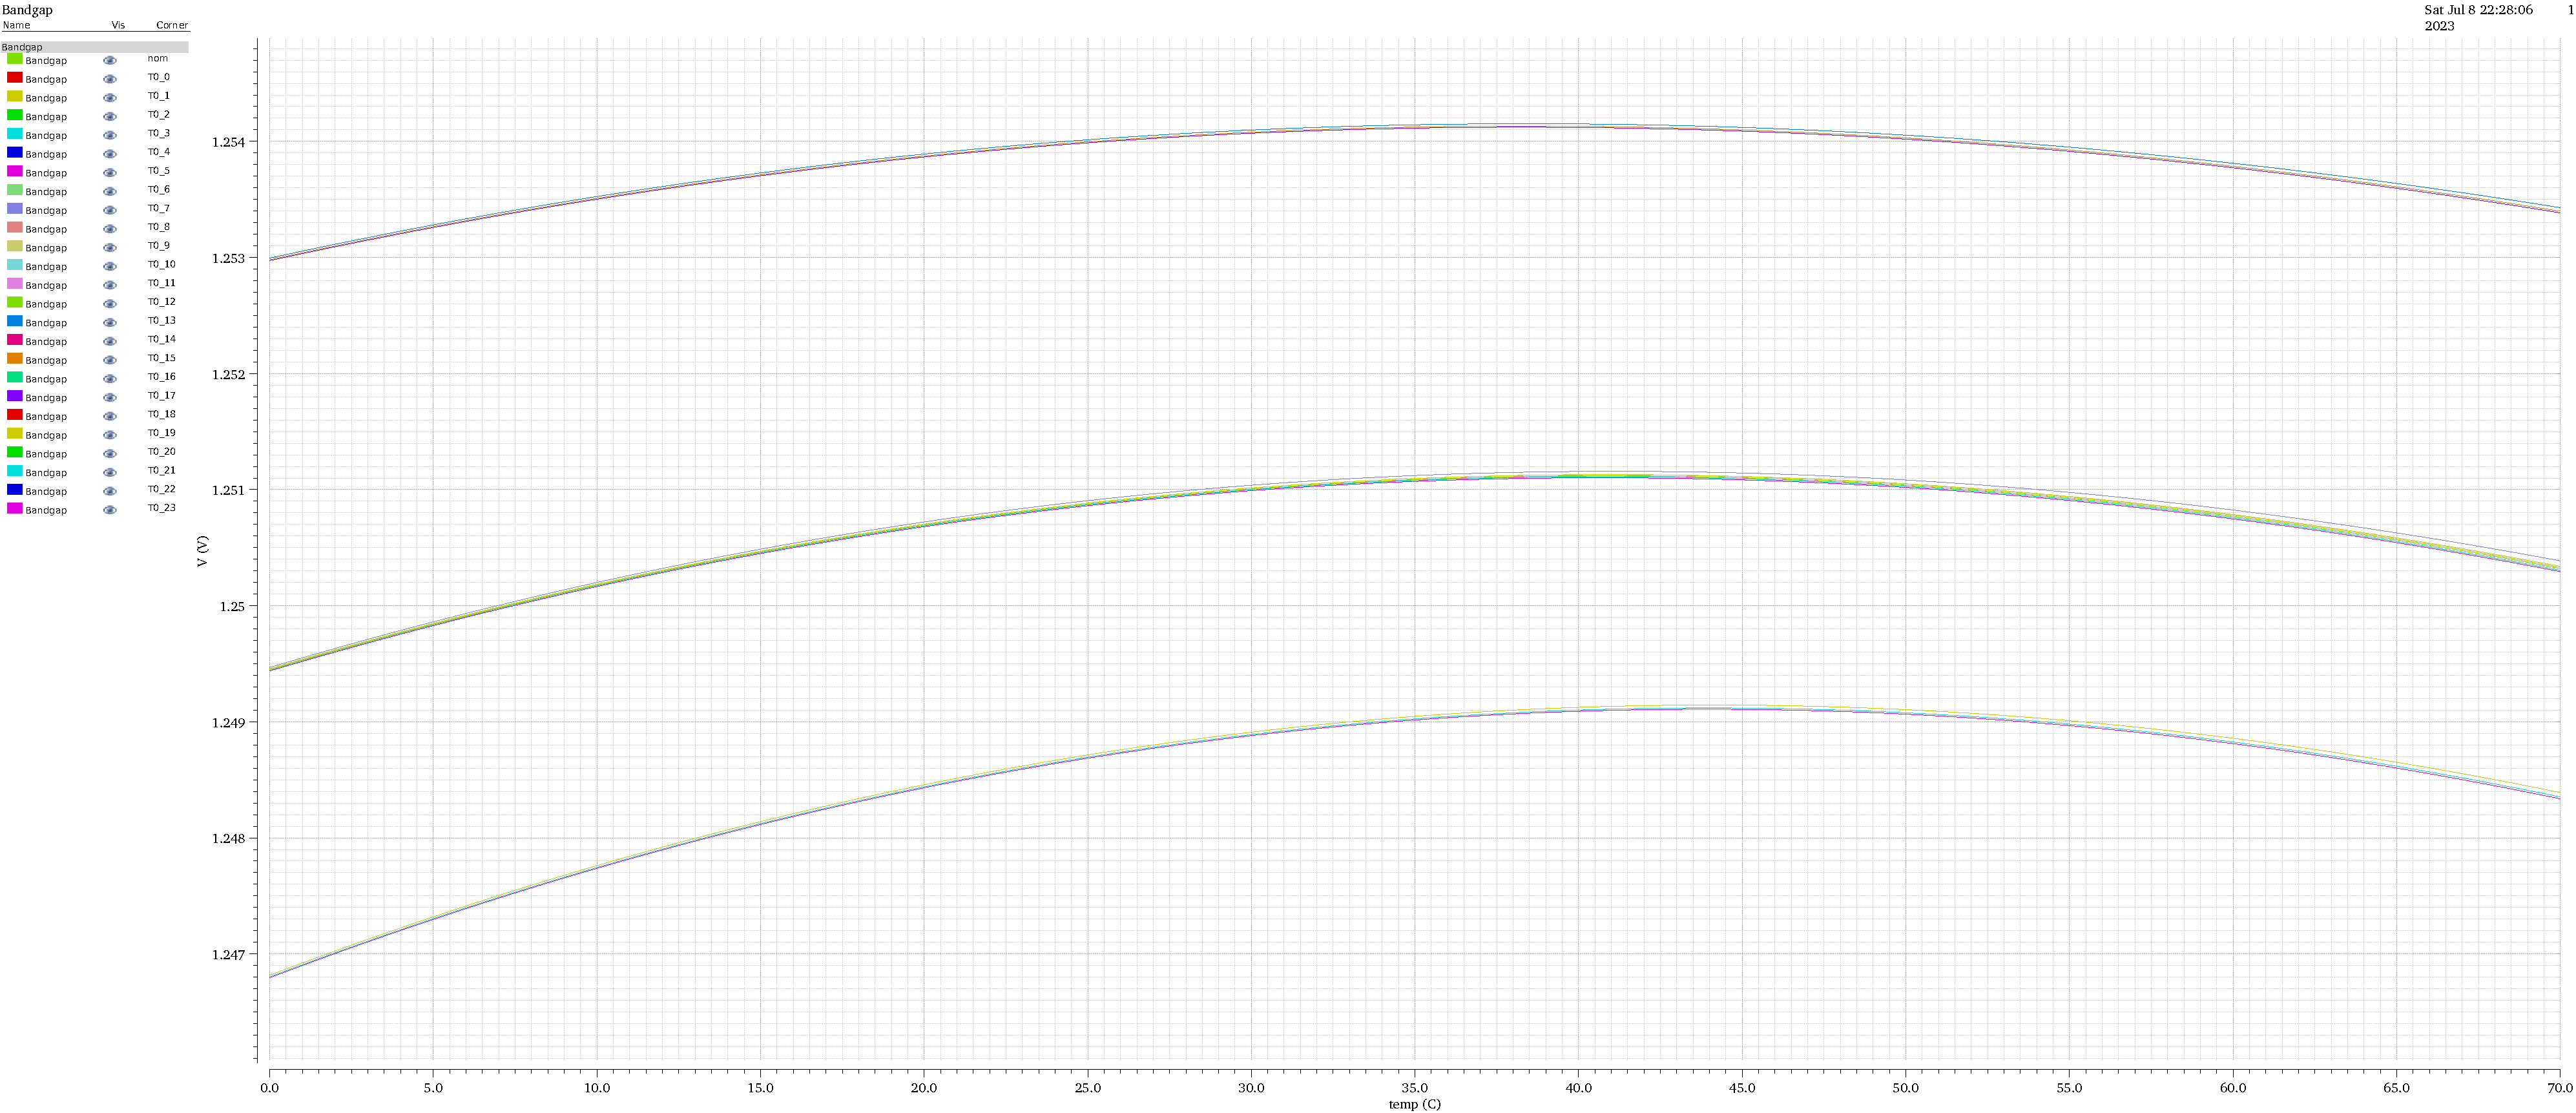
\includegraphics[width=\textwidth]{images/05_bandgap/band_volt.pdf}
	\caption{Bandgap voltage vs temperature simulated}
	\label{fig:bandgap_voltage_vs_temp}
\end{figure}
\begin{figure}[ht]
	\centering
	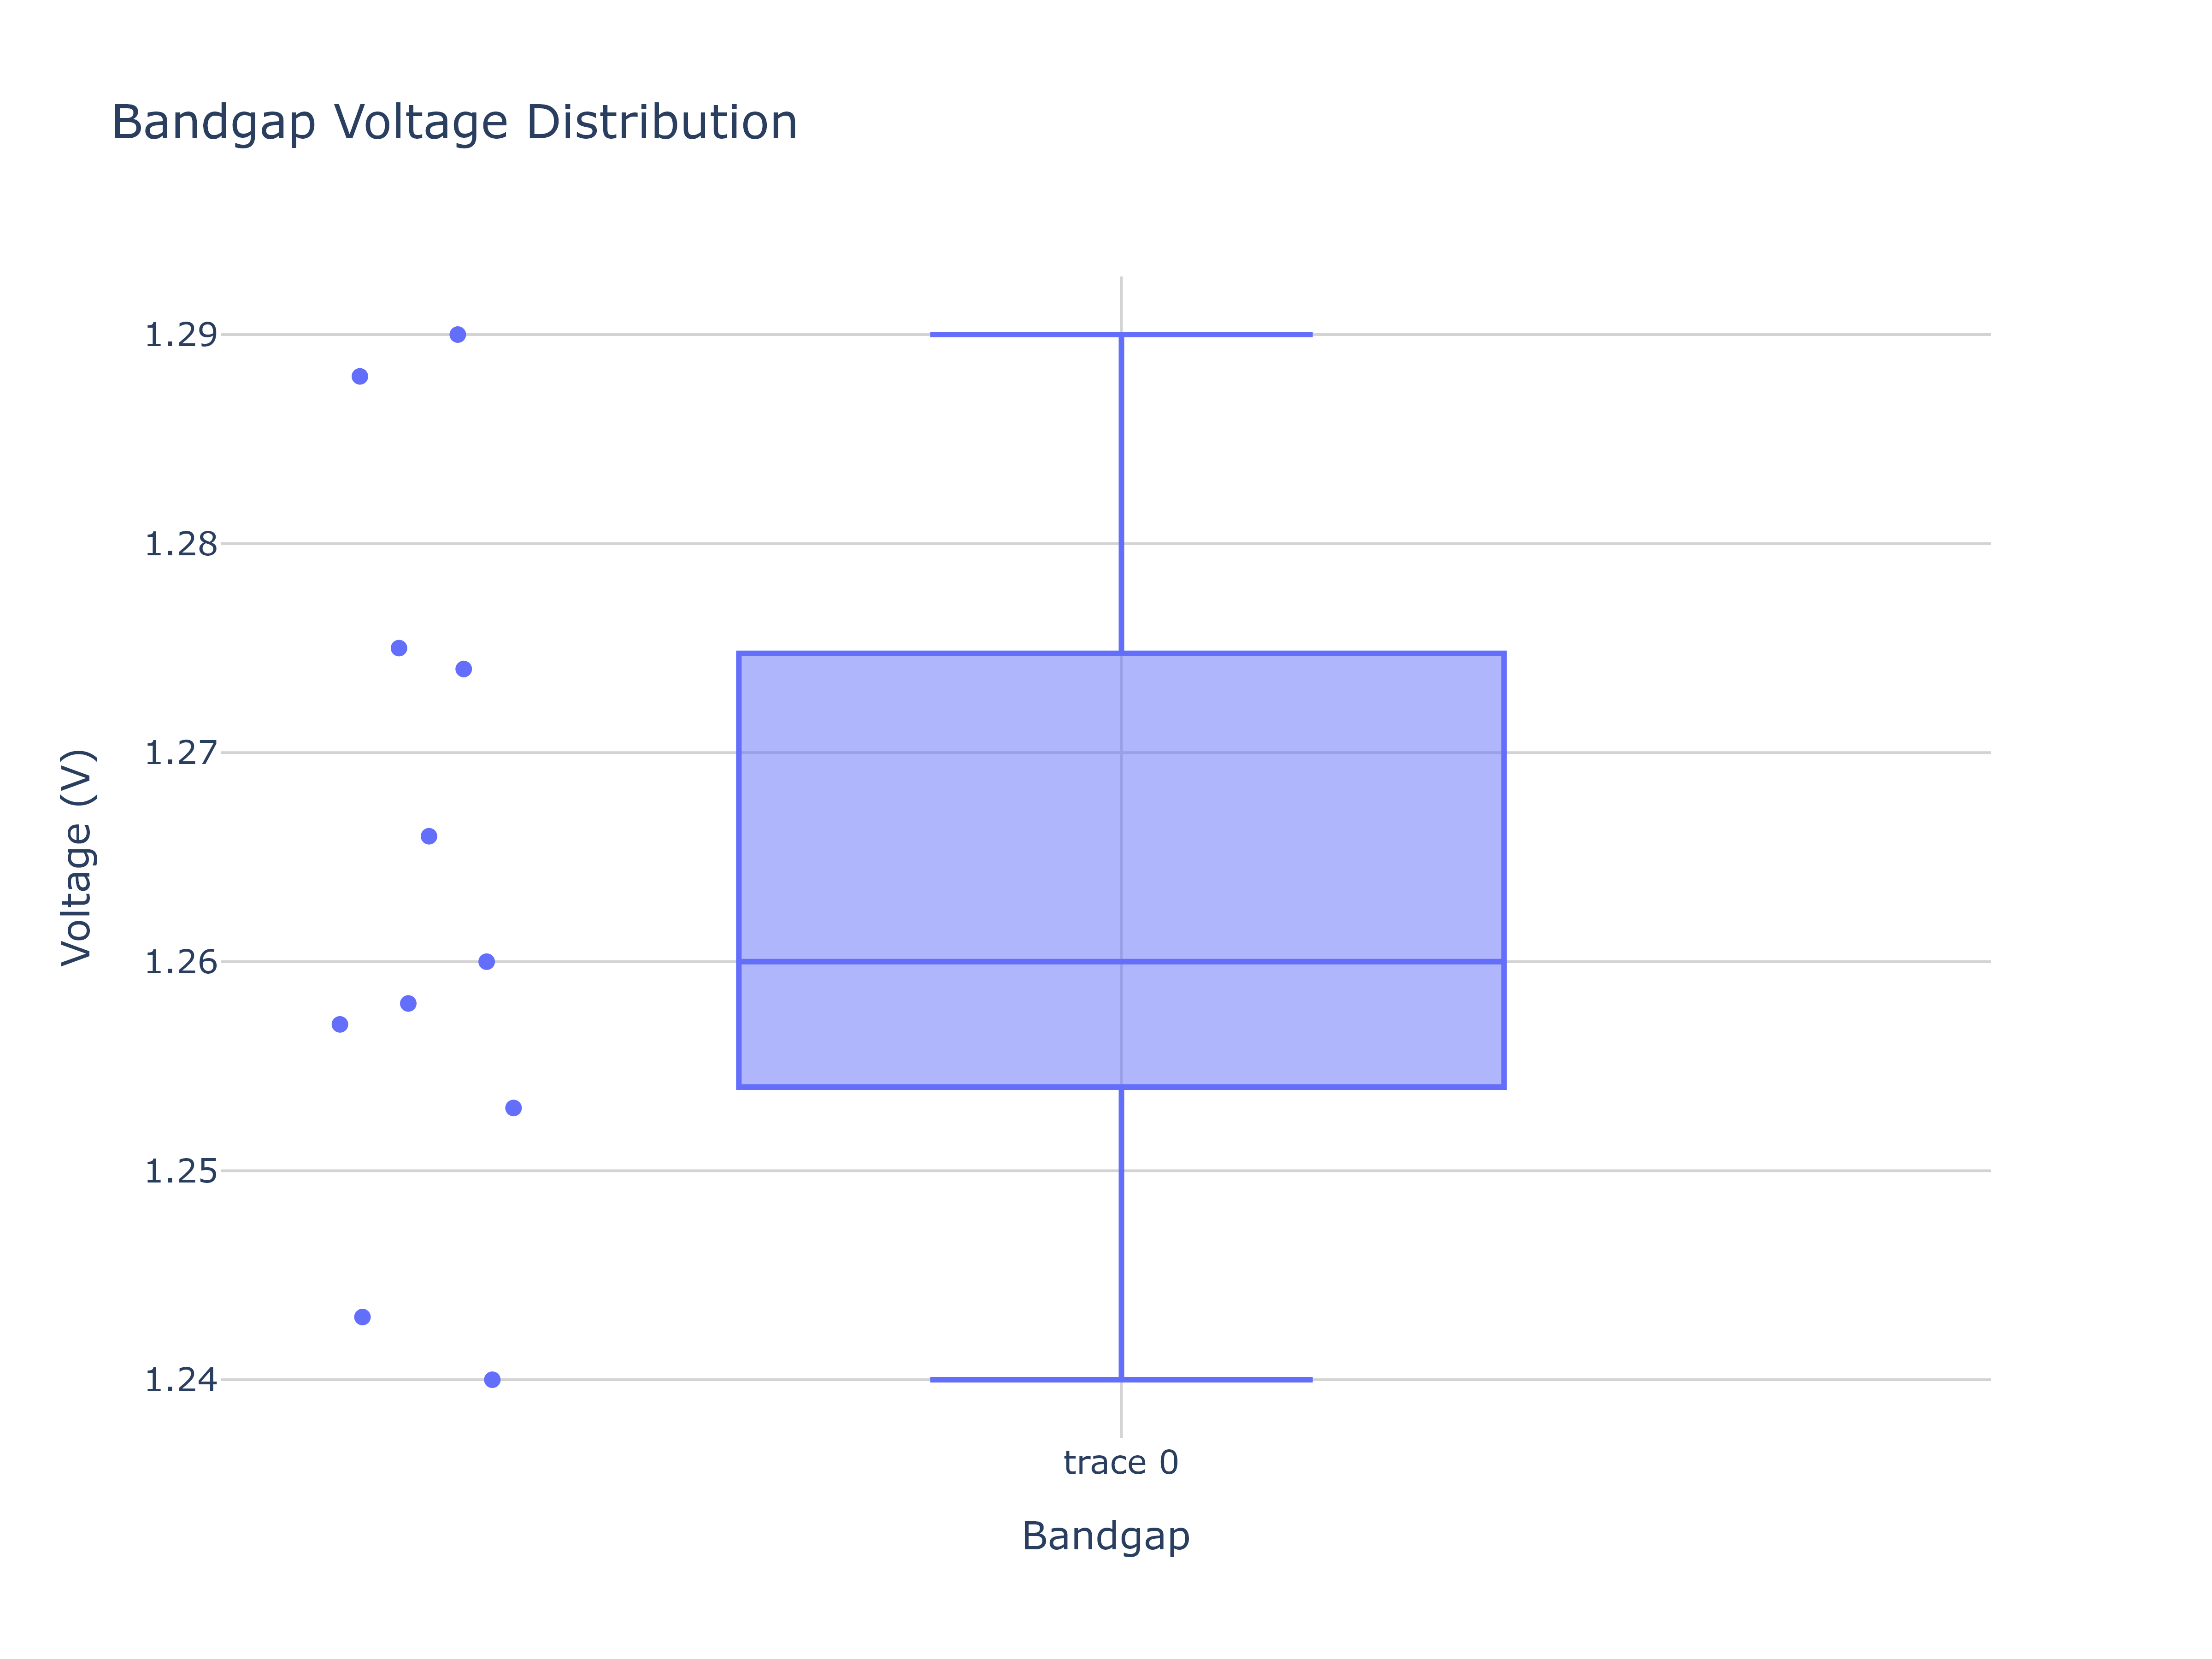
\includegraphics[width=\textwidth]{images/Bandgap_Voltage_Distribution.png}
	\caption{Bandgap voltage distribution at 22 degree Celsius}
	\label{fig:bandgap_voltage_distrb}
\end{figure}

\begin{figure}[ht]
	\centering
	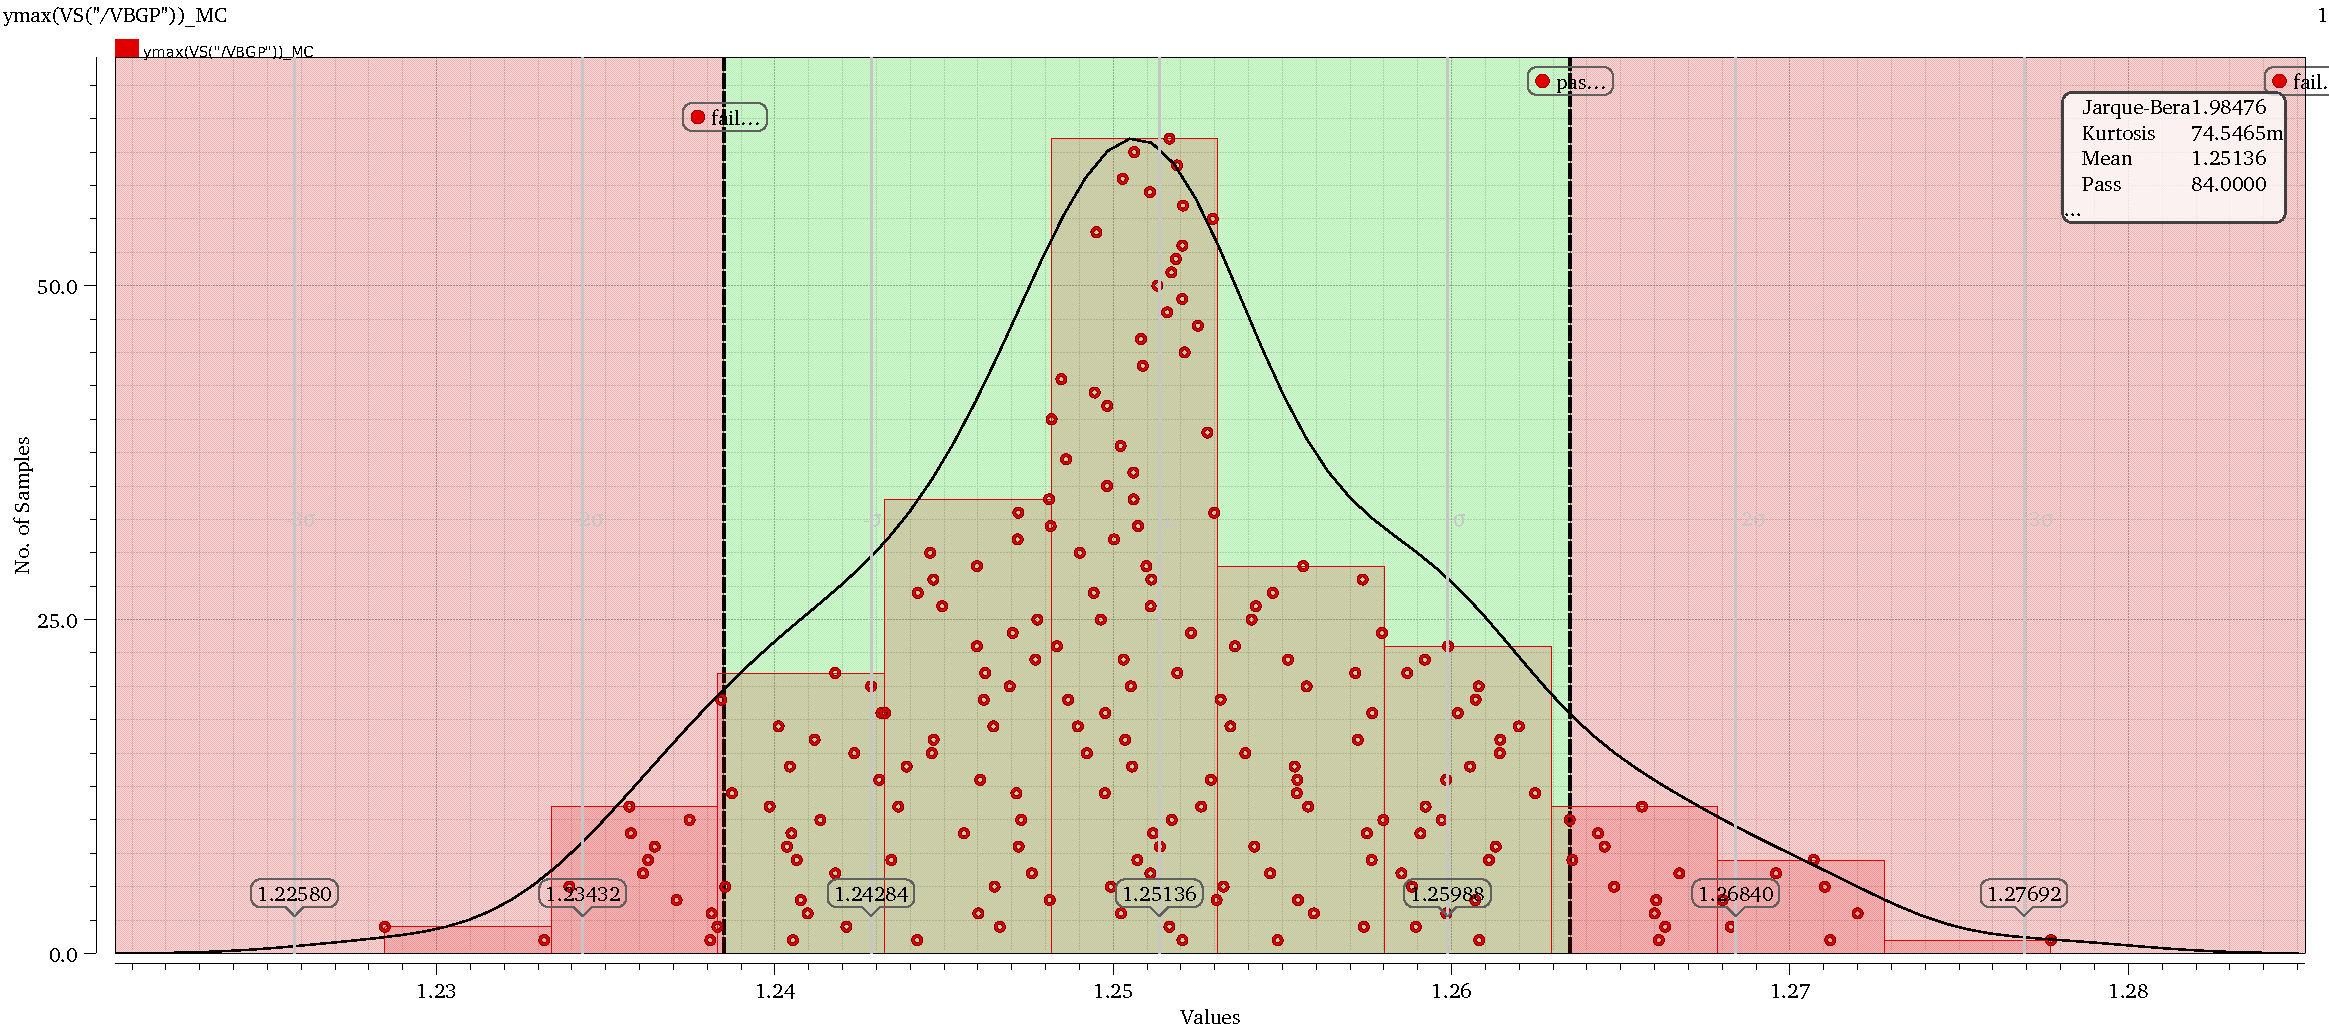
\includegraphics[width=\textwidth]{images/05_bandgap/band_volt_mc.pdf}
	\caption{Bandgap voltage Monte Carlo simulation (param.scs=3s, xh035.scs=mcg)}
	\label{fig:bandgap_voltage_mc}
\end{figure}
\clearpage
\subsection{Current Source}
The current source characteristics from the simulation can be seen in \autoref{tab:current_source} and \autoref{fig:current_source}. The measurements have thereby shown that the current source is in the range of of the simulation. The current was measured for one chip and its value was thereby \textcolor{red}{10 micro ampere}. About the other parameters no measurements could be done since the current source is not directly accessible.
\begin{longtable}{|p{3.5cm}|p{3.5cm}|p{3.5cm}|p{3.5cm}|}
	\hline
	\rowcolor{lightgray}
	\textbf{Description} &\textbf{Min} &\textbf{Max} & \textbf{Unit} \\ \hline
	
	Reference current & 8.4 & 13.5 &\qty{}{\micro\ampere} \\ \hline
	Current consumption & 50 & 81 & \qty{}{\micro\ampere} \\ \hline
	Min voltage (voltage where the trans resistance ($\frac{\Delta V_{in}}{\Delta I_{out}}$) is higher than \qty{1}{\mega\ohm}) & 3& 3.33 & \qty{}{\volt} \\ \hline
	\caption{Current reference characteristics} % needs to go inside longtable environment
	\label{tab:bootstrap}
\end{longtable}
\begin{figure}[ht]
	\centering
	
	\resizebox{1\textwidth}{!}{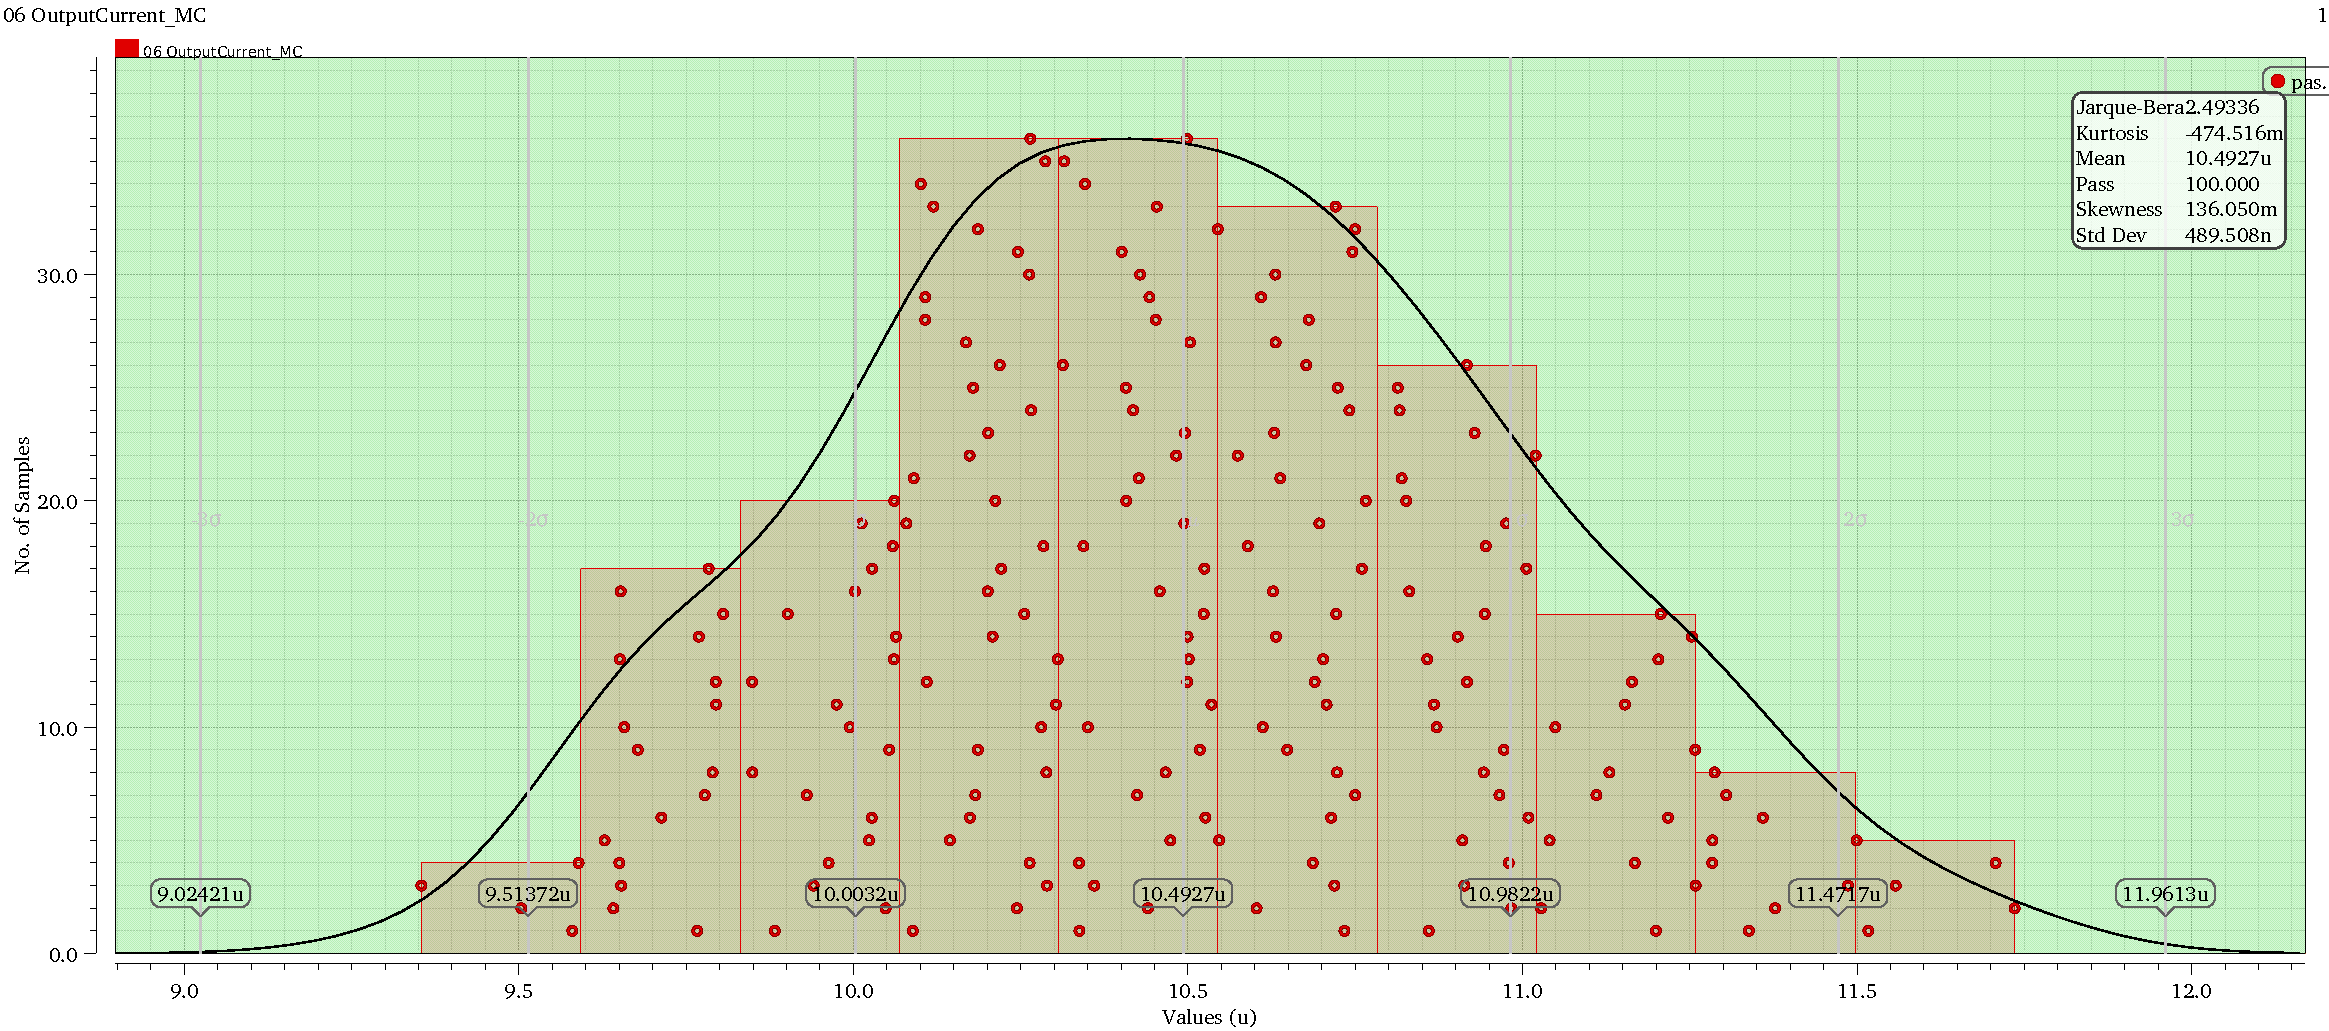
\includegraphics{images/06_current_ref/ref_cur_mont.pdf}}
	\caption{Monte Carlo distribution of Current reference. X-axis shows current through \glqq IPRB0\grqq{} in \autoref{fig:ref_cur_sim_schem} (param.scs=3s, xh035.scs=mcg)}
	\label{fig:ref_cur_mont}
\end{figure}
\begin{figure}[ht]
	\centering
	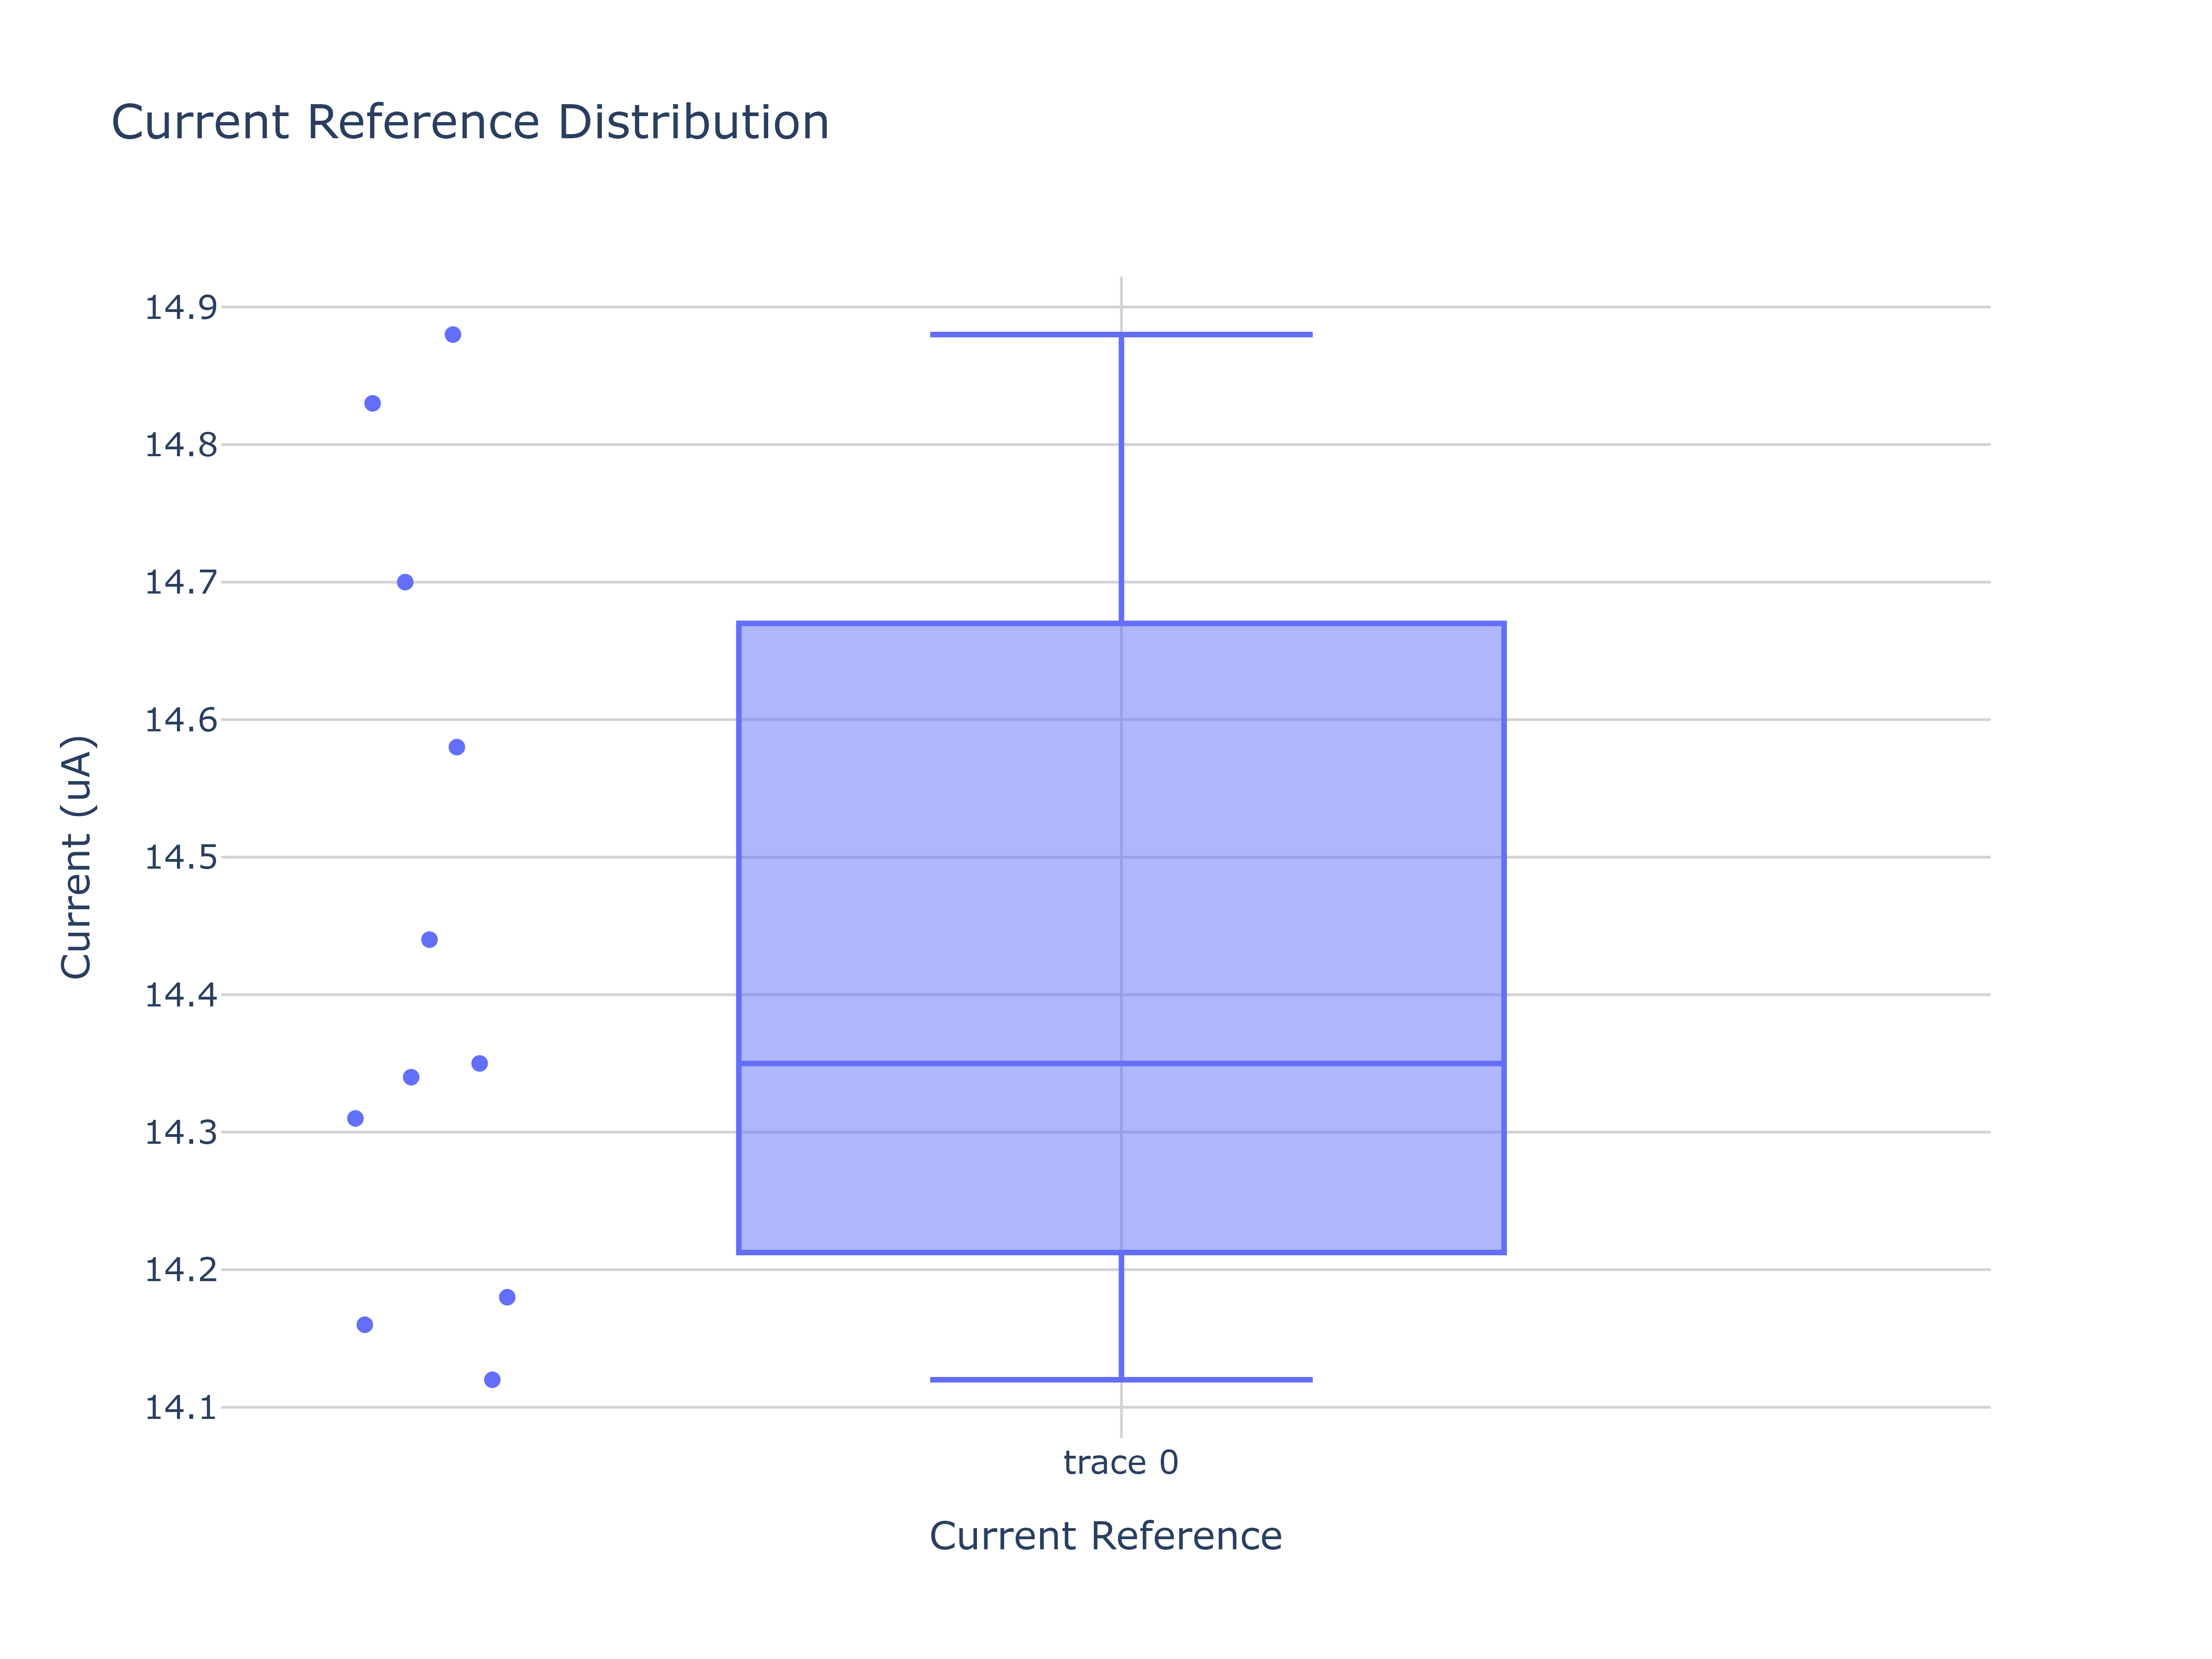
\includegraphics[width=\textwidth]{images/Current_Reference_Distribution.png}
	\caption{Current source distribution at 22° degree Celsius}
	\label{fig:current_source_distr}
\end{figure}
\clearpage
\subsection{Oscillator}
The oscillator characteristics from the simulation can be seen in \autoref{tab:osc} and \autoref{fig:osc}. The measurements have thereby shown that the oscillator is in the range of of the simulation. The frequency was measured for one chip and its value was thereby \textcolor{red}{1.5 \qty{}{\mega\hertz}}. About the other parameters no measurements could be done since the oscillator is not directly accessible. Furthermore the frequency could also be tuned in the range of \textcolor{red}{x to y} over the spi registers. 
\begin{longtable}{|p{3.5cm}|p{3.5cm}|p{3.5cm}|p{3.5cm}|}
	\hline
	\rowcolor{lightgray}
	\textbf{Description} &\textbf{Min} &\textbf{Max} & \textbf{Unit} \\ \hline
	
	Frequency & 1.15 & 1.7 &\qty{}{\mega\hertz} \\ \hline
	Current consumption & 35 & 50 & \qty{}{\micro\ampere} \\ \hline
	Min voltage & 2& 3.187 & \qty{}{\volt} \\ \hline
	\caption{Specification} % needs to go inside longtable environment
	\label{tab:osc}
\end{longtable}

\clearpage


\subsection{Buck-Boost Converter}

\subsubsection{Start-up}
\label{sec:startup}
The start-up behavior shows significant differences to the results observed in simulations. Instead of the expected gradual increase in the output voltage, we observed the output voltage increase in distinct steps as can be seen in \autoref{fig:startup}. These distinct steps stem from the fact the input voltage collapses cyclicly to under the limit given by the \ac{POR}. The cycle can be described as the chip starting up and increasing the input current until the input voltage drops to bellow the limit given by the \ac{POR} thus disabling the chip and causing the input voltage to rise until the chip starts up again. The cycle continues until the output voltage reaches close to the nominal level and the outer voltage control loop regulates the current.  
The underlying issue is a misconfiguration of the internal registers causing the current limit to be disabled on start-up and the converter increasing the inductor current $I_L$ to unsustainable levels leading to the collapse of the input voltage. The cause is further described in \autoref{sec:missingcurrentlimit}.

\begin{figure}[ht]
	\centering
	
	\resizebox{1\textwidth}{!}{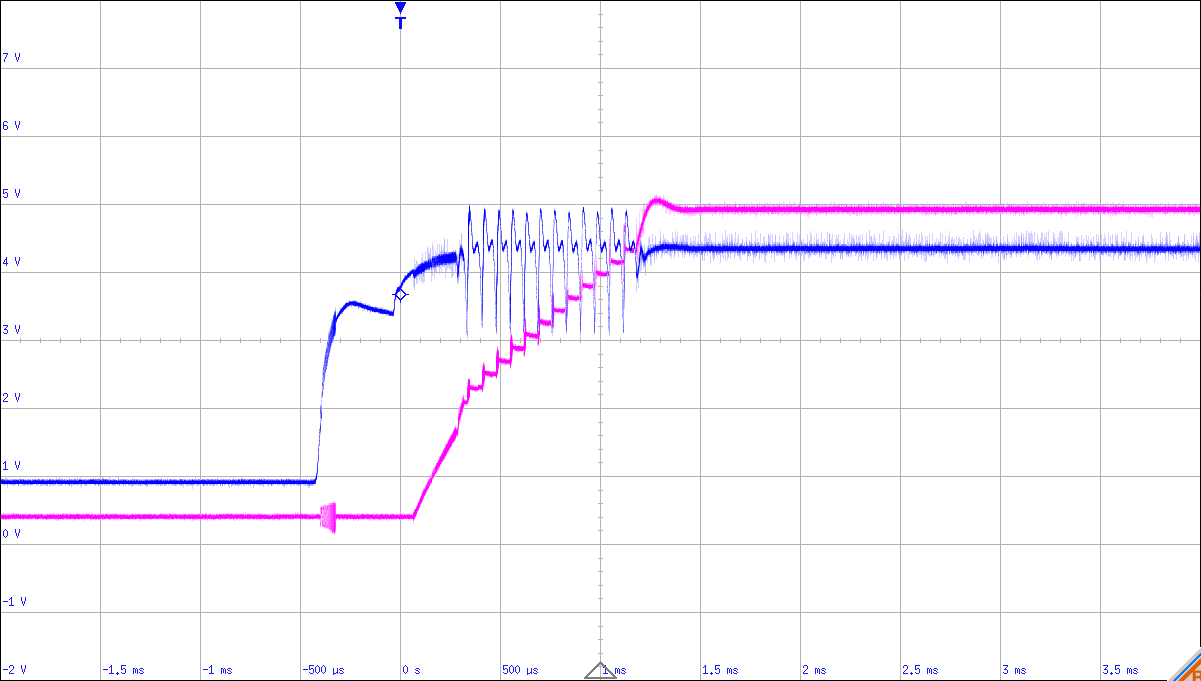
\includegraphics{images/07_DCDC/StartUp.PNG}}
	\caption{Start-up behavior without an attached load. Dark Blue: $V_{IN}$ measured; Pink: $V_{OUT}$ measured}
	\label{fig:startup}
\end{figure}


\subsubsection{Load Step Response}
The response to a load step is satisfactory and can be seen \autoref{fig:loadstep}. The regulation behavior is similar to the simulated response, but the measured controller has a higher bandwidth as can be seen in the faster response and is slightly overcompensated as it lacks the single oscillatory peak seen in the simulated response. Based on this response we estimate the implemented system has the following characteristics:

\begin{table}[H]
    \centering
    \begin{tabular}{|c|c|c|}
        Characteristic & Measured System & Simulation \\
        \hline
         Phase Margin  & \qty{55}{\degree} & \qty{45}{\degree}\\
		 Crossover Frequency & \qty{30}{\kilo\hertz} & \qty{20}{\kilo\hertz}  \\
    \end{tabular}
    \caption{Estimated regulator characteristics based on the response to a 200 mA load step}
    \label{tab:regChar}
\end{table}

\begin{figure}[ht]
	\centering
	
	\resizebox{1\textwidth}{!}{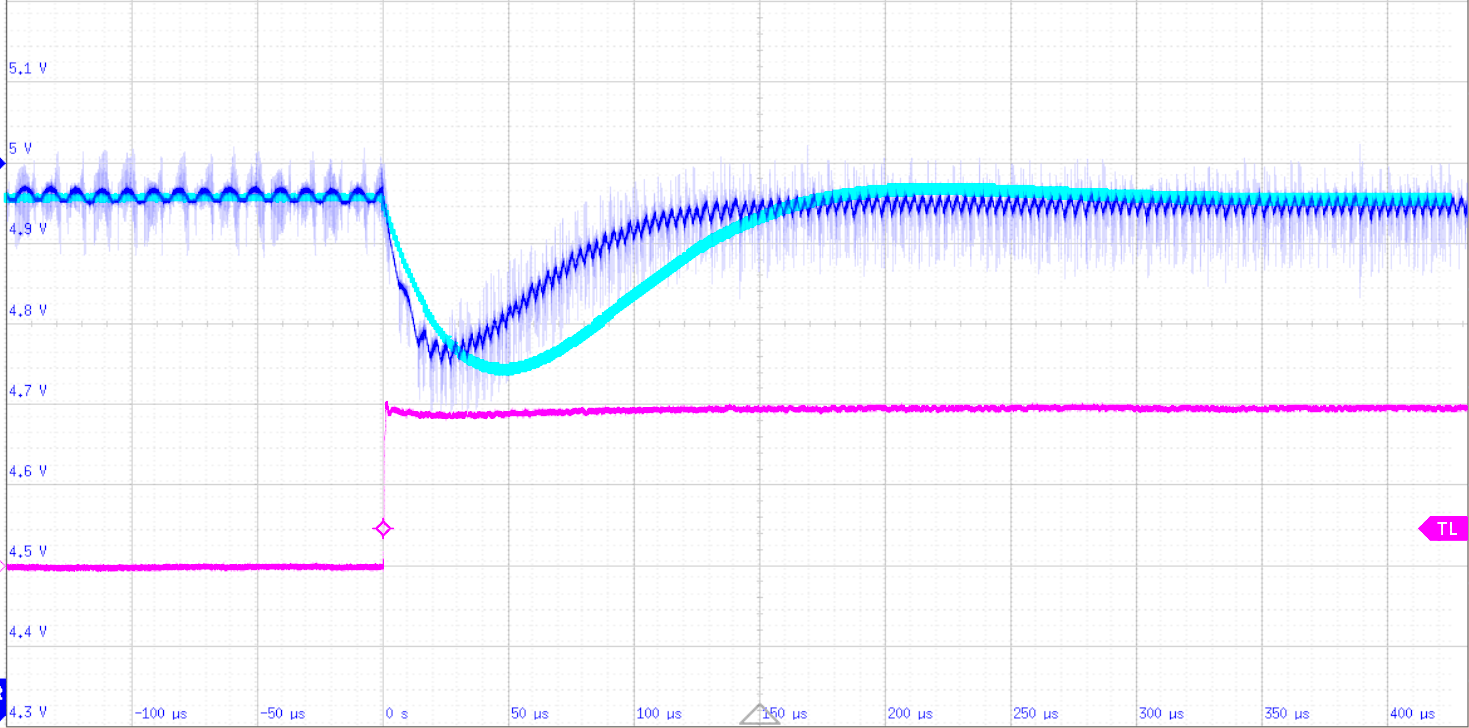
\includegraphics{images/07_DCDC/LoadStepVergleich.png}}
	\caption{Load regulation to a 200 mA load step for comparison between measured response and simulated response. Simulated response offset to remove constant load regulation error. Dark Blue: $V_{OUT}$ measured; Light Blue: $V_{OUT}$ simulated; Pink: $I_{OUT}$ measured}
	\label{fig:loadstep}
\end{figure}
\clearpage

\subsubsection{Load Regulation}
\label{sec:loadRegulation}
\begin{figure}[ht]
	\centering
	\resizebox{1\textwidth}{!}{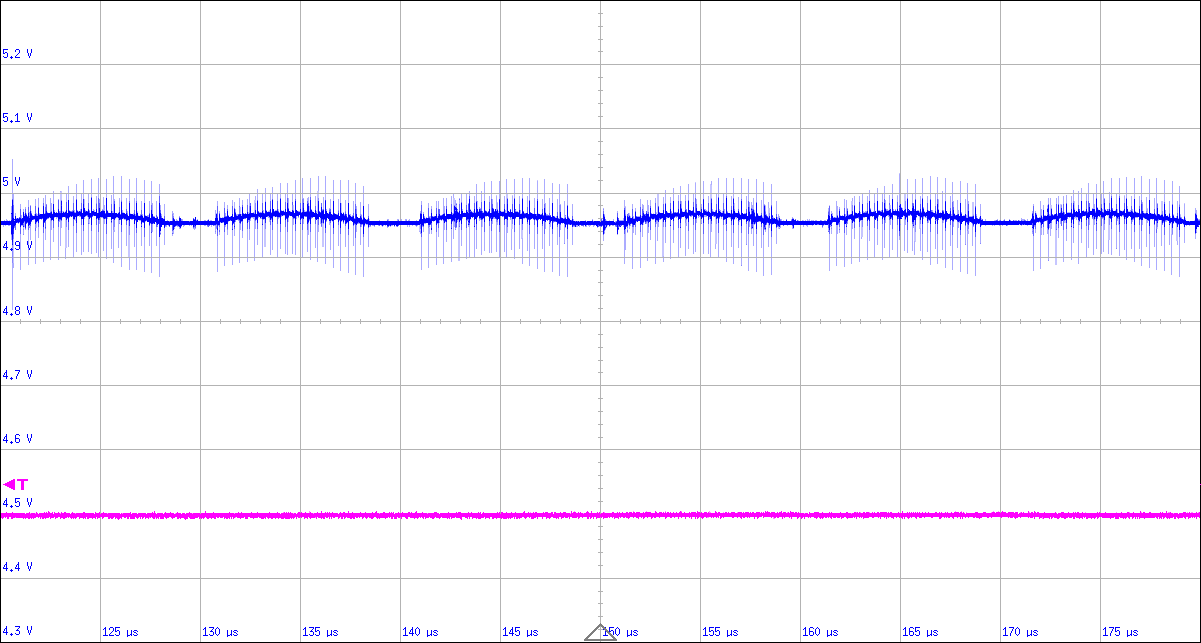
\includegraphics{images/07_DCDC/LoadSteadyState0mA.png}}
	\caption{Steady state load regulation with a 0mA load. Dark Blue: $V_{OUT}$; Pink: $I_{OUT}$}
\end{figure}
\begin{figure}[ht]
	\centering
	\resizebox{1\textwidth}{!}{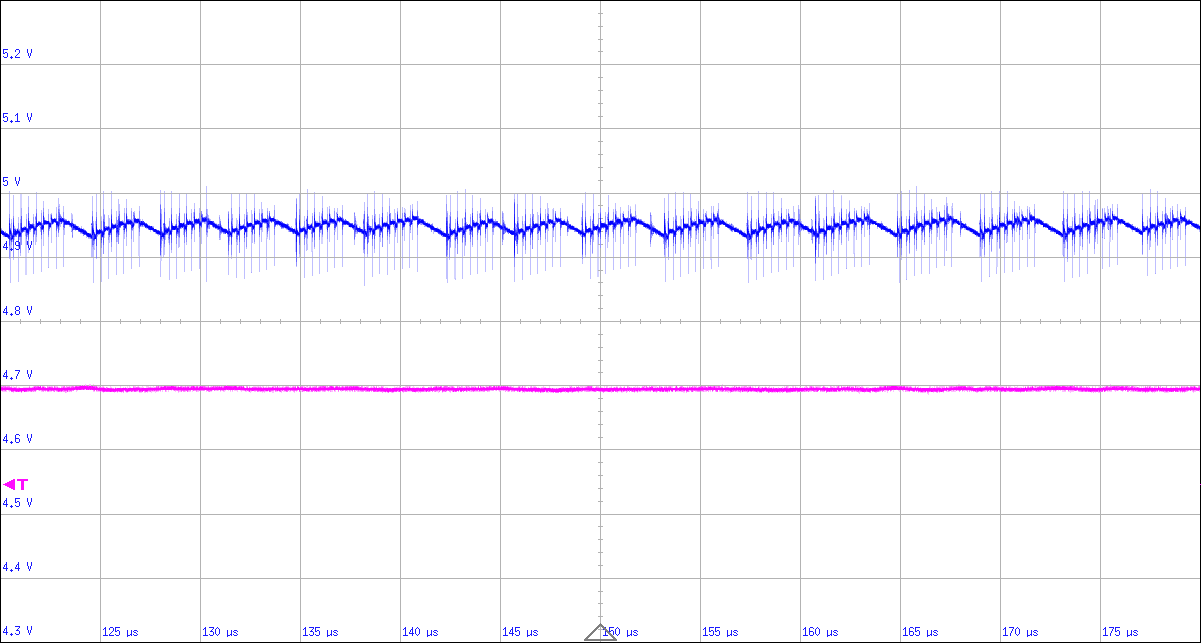
\includegraphics{images/07_DCDC/LoadSteadyState200mA.png}}
	\caption{Steady state load regulation with a 200mA load. Dark Blue: $V_{OUT}$; Pink: $I_{OUT}$}
\end{figure}
\clearpage



\foreach \i in {../ASIC-DESIGN-2/images/03_plots/DCDC Reset Test with 4.3V and resistor R2\, 70°C} {
    \begin{figure}[h]
        \centering
    \includegraphics[width=0.95\textwidth]{\i.pdf}
    %     \caption{\i}
    \end{figure}
    
}
\subsubsection{Efficiency}
The efficiency of the TI chip was measured at different input voltages and loads. The efficiency was thereby callculated by difiding the output power by the input power. The results can be seen in \autoref{fig:efficiency TI chip}.
\begin{figure}[h]
    \centering
    \includegraphics[width=0.8\textwidth]{../ASIC-DESIGN-2/images/03_plots/efficiencyTI.pdf}
    \caption{Efficiency TI CHIP}
    \label{fig:efficiency TI chip}
\end{figure}
